\begin{frame}[t]{\secname}{\subsecname{}}

% Styles
\tikzset{
  failurespy style/.style={
    spy scope={%
      failurespyscope style,%
    },
    connect spies/.style={
      failurespyconnect style,%
    },
  }
}

\tikzset{
  failurespyscope style/.style={
    magnification=4,
    connect spies,                            % Connect orig. & detail
    width=0.45\linewidth,                     % Spy width
    height=0.40\linewidth,                    % Spy height
    every spy on node/.style={                % Source
      rectangle,                              % Form
      rounded corners=0.004\linewidth,        % Edge shape
      dashed,                                 % Dashed line
      draw=black,                             % Line color
      %thick,                                  % Line style for spy
    },
    every spy in node/.style={                % Spy
      rectangle,                              % Form
      rounded corners=0.004\linewidth,        % Edge shape
      dashed,                                 % Dashed line
      draw=black,                             % Line color
      %thick,                                  % Line style for spy
    },
  },
}

\tikzset{
  failurespyconnect style/.style={
    spy connection path={
      \draw[%
        %thick,
        dashed,
        black
      ] (tikzspyonnode) -- (tikzspyinnode); % In-On-Connection
    },
  },
}

\begin{columns}[t]
  \begin{column}{0.5\textwidth}
    \begin{itemize}
      \item Bond-based critical stretch models: \\[0.5ex]
      \begingroup
      \small 
        \begin{tabular}{@{}lc@{}}
          $\epsilon_{c}=\sqrt{\dfrac{5G_c}{9K\delta}}$&\cite{SillingSA2005,BobaruF2017}\\[2ex]%\tabto{5.5cm}
          $\epsilon_{c}=\sqrt{\dfrac{G_c}{\left[3G+\left(\frac34\right)^4\left(K-\frac{5G}{3}\right)\right]\delta}}$&\cite{MadenciE2014}%\tabto{5.5cm}
        \end{tabular}
      \endgroup
      \item<1-> Based on Griffith for existing pre-crack
      \item<1-> $\epsilon_{c}=f\left(\delta^{-\frac12}\right)$
      \item<2-> Reproducibility for various $\delta$ and adapted $\epsilon_c$ in SB-PD 1D-case for no pre-crack?%of failure displacement
      
    \end{itemize}
  \end{column}
  \begin{column}{0.5\textwidth}
    \only<3-4|handout:1-2>{
      \begin{block}{Hex, $dx=\SI{0.4}{\milli\meter}$}
        \only<3|handout:1>{
          % Data
          \pgfplotstableread[col sep=comma]{\materialpath/Data/Numerics/Hex_0-4_CritStretch.csv}{\loadedtable}
          % Dimensions
          \setlength{\figwidth}{\linewidth}
          \setlength{\figheight}{0.75\textheight}
          % Chart
          \tikzexternalenable
          \tikzsetnextfilename{Hex_0-4_CritStretch}
          \begin{tikzpicture}
            \begin{axis}[
              height=\figheight,
              width=\figwidth,
              axis lines=middle,
              cycle list name=color list,%linestyles*,
              cycle list shift=1,
              xmin=0,
              ymin=0,
              title=\empty,
              xlabel={$u$ $[\si{\milli\meter}]$},
              ylabel={$F$ $[\si{\newton}]$},
              label style={font=\figurefontsize},
              %x label style={at={(axis description cs:0.5,-0.075)},anchor=north},
              %y label style={at={(axis description cs:-0.085,0.5)},rotate=90,anchor=south},
              legend pos=south west,
              legend cell align={left},
              legend style={font=\figurefontsize},
              ticklabel style={font=\figurefontsize},
            ]%   each nth point={2}
    %           %\addplot+ table[x=Dx5, y=Fx5] {\loadedtable};
    %           %\addlegendentry{$\delta=\SI{5}{\milli\meter}$, $\epsilon_c=\num[round-mode=places,round-precision=2]{9.797959e-3}$}
    %           %\addplot+ [] table[x=Dx4, y=Fx4] {\loadedtable};
    %           %\addlegendentry{$\delta=\SI{4}{\milli\meter}$, $\epsilon_c=\num[round-mode=places,round-precision=2]{1.0954451e-2}$}
              \addplot+ [] table[x=Dx3, y=Fx3] {\loadedtable};
              \addlegendentry{$\delta=\SI{3}{\milli\meter}$}%, $\epsilon_c=\num[round-mode=places,round-precision=2]{1.2649111e-2}$}
              \addplot+ [] table[x=Dx2, y=Fx2] {\loadedtable};
              \addlegendentry{$\delta=\SI{2}{\milli\meter}$}%, $\epsilon_c=\num[round-mode=places,round-precision=2]{1.5491933e-2}$}
              \addplot+ [] table[x=Dx1.5, y=Fx1.5] {\loadedtable};
              \addlegendentry{$\delta=\SI{1.5}{\milli\meter}$}%, $\epsilon_c=\num[round-mode=places,round-precision=2]{1.7888544e-2}$}
    %           \pgfplotsset{cycle list shift=2} % Jump one in cycle - 1.25
              \addplot+ [] table[x=Dx1.2, y=Fx1.2] {\loadedtable};
              \addlegendentry{$\delta=\SI{1.2}{\milli\meter}$}%, $\epsilon_c=\num[round-mode=places,round-precision=2]{2e-2}$}
              \pgfplotsset{cycle list shift=1} % Jump one in cycle - 1.18
              \addplot+ [] table[x=Dx1, y=Fx1] {\loadedtable};
              \addlegendentry{$\delta=\SI{1}{\milli\meter}$}%, $\epsilon_c=\num[round-mode=places,round-precision=2]{2.1908902e-2}$}
              \addplot+ [] table[x=Dx0.875, y=Fx0.875] {\loadedtable};
              \addlegendentry{$\delta=\SI{0.875}{\milli\meter}$}%, $\epsilon_c=\num[round-mode=places,round-precision=2]{2.3421602e-2}$}
            \end{axis}
          \end{tikzpicture}
          \tikzexternaldisable
%             \includegraphics[width=\figwidth,height=\figheight,keepaspectratio]{example-image-a}           
        }
        \only<4|handout:2>{
          \setlength{\figheight}{0.55\textheight}
          \vspace{1ex}
          \figurefontsize
          \begin{minipage}[t][0.65\textheight][t]{0.49\linewidth}
            \centering
            \tikzexternalenable
            \tikzsetnextfilename{PD_Hex_Damage_0-4_1-2_3630_-z_spy}
            \begin{tikzpicture}[
              failurespy style,
            ]
              \node[inner sep=0] (PDHex1) {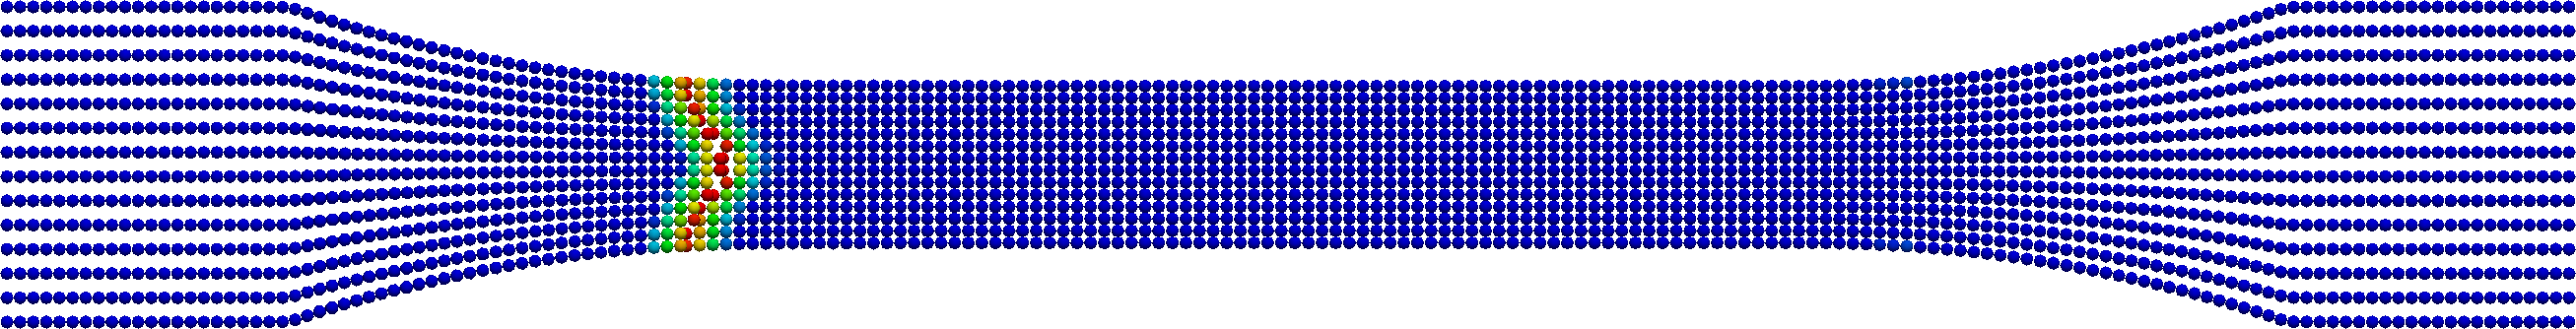
\includegraphics[angle=90,width=\linewidth,height=\figheight,keepaspectratio]{PD_Hex_Damage_0-4_1-2_3630_-z_ct.png}};
              \begin{scope}[
                shift={(PDHex1.south west)},
                x={(PDHex1.south east)},
                y={(PDHex1.north west)},
              ]
                \coordinate (spypointpdhex1) at (0.5,0.275);
                \coordinate (spyviewerpdhex1) at (1.0,0.5);
                \spy on (spypointpdhex1) in node[anchor=west] at (spyviewerpdhex1);
              \end{scope}
            \end{tikzpicture}\\
            \tikzexternaldisable
            $\delta=\SI{1.2}{\milli\meter}$
          \end{minipage}
          \begin{minipage}[t][0.65\textheight][t]{0.49\linewidth}
            \centering
            \tikzexternalenable
            \tikzsetnextfilename{PD_Hex_Damage_0-4_2_3955_-z_spy}
            \begin{tikzpicture}[
              failurespy style,
            ]
              \node[inner sep=0] (PDHex2) {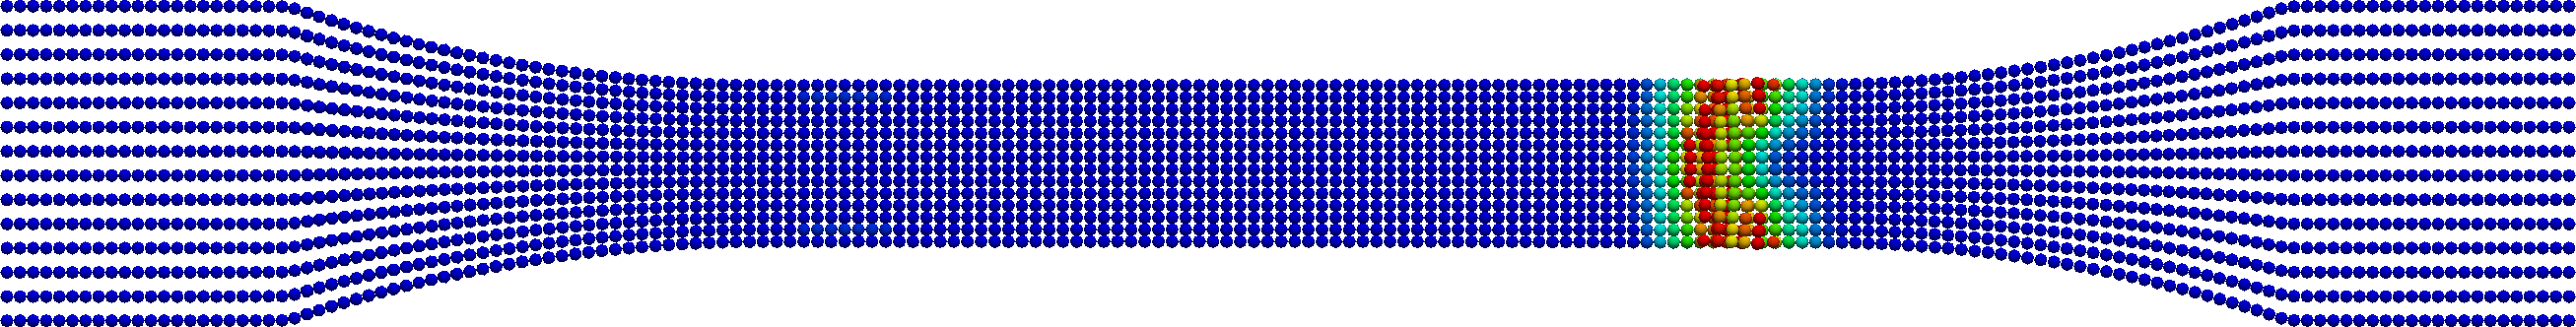
\includegraphics[angle=90,width=\linewidth,height=\figheight,keepaspectratio]{PD_Hex_Damage_0-4_2_3955_-z_ct.png}};
              \begin{scope}[
                shift={(PDHex2.south west)},
                x={(PDHex2.south east)},
                y={(PDHex2.north west)},
              ]
                \coordinate (spypointpdhex2) at (0.5,0.67);
                \coordinate (spyviewerpdhex2) at (1.0,0.5);
                \spy on (spypointpdhex2) in node[anchor=west] at (spyviewerpdhex2);
              \end{scope}
            \end{tikzpicture}\\
            \tikzexternaldisable
            $\delta=\SI{2}{\milli\meter}$
          \end{minipage}
        }
      \end{block}
    }
    \only<5-|handout:3>{
      \begin{block}{Tet, $dx=\SI{0.5}{\milli\meter}$}
        %\only<3|handout:0>{
          \setlength{\figheight}{0.55\textheight}
          \vspace{1ex}
          \figurefontsize
          \begin{minipage}[t][0.65\textheight][t]{0.49\linewidth}
            \centering
            \tikzexternalenable
            \tikzsetnextfilename{PD_Tet_Damage_0-5_0-5625_9600_-z_spy}
            \begin{tikzpicture}[
              failurespy style,
            ]
              \node[inner sep=0] (PDTet1) {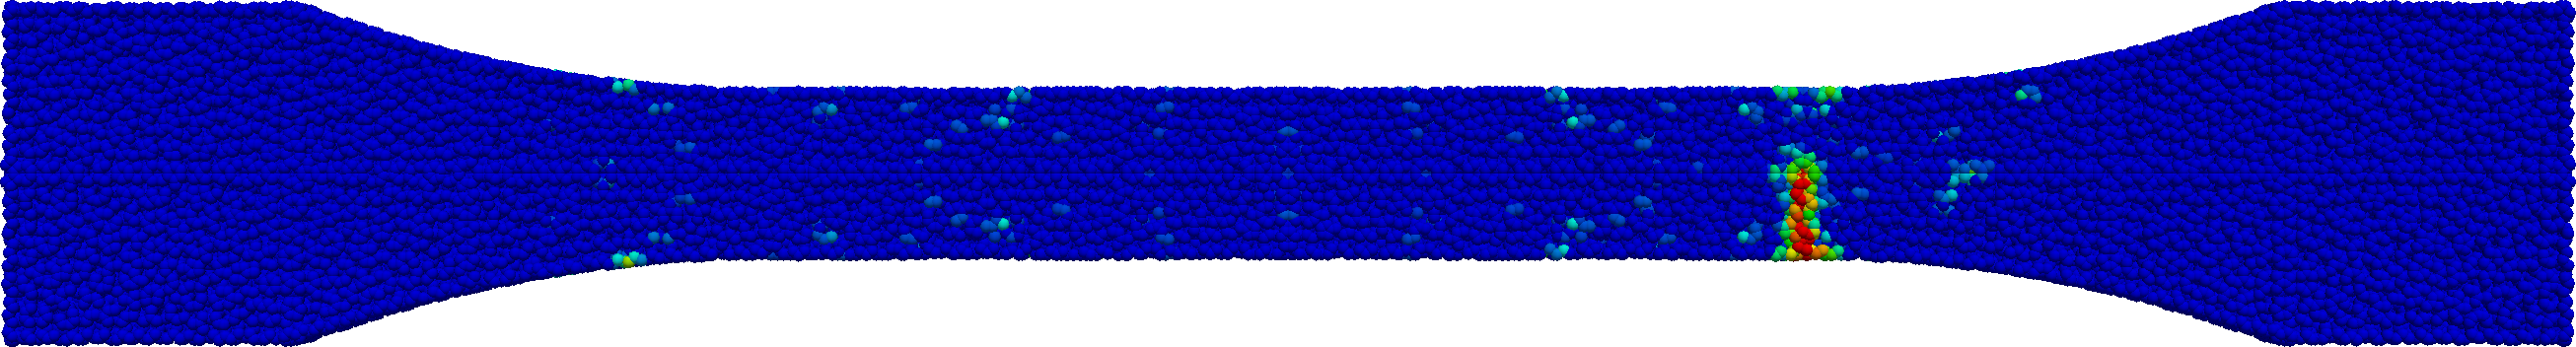
\includegraphics[angle=90,width=\linewidth,height=\figheight,keepaspectratio]{PD_Tet_Damage_0-5_0-5625_9600_-z_ct.png}};
              \begin{scope}[
                shift={(PDTet1.south west)},
                x={(PDTet1.south east)},
                y={(PDTet1.north west)},
              ]
                \coordinate (spypointpdtet1) at (0.5,0.700);
                \coordinate (spyviewerpdtet1) at (1.0,0.5);
                \spy on (spypointpdtet1) in node[anchor=west] at (spyviewerpdtet1);
              \end{scope}
            \end{tikzpicture}\\
            \tikzexternaldisable
            $\delta=\SI{0.56}{\milli\meter}$
          \end{minipage}
          \begin{minipage}[t][0.65\textheight][t]{0.49\linewidth}
            \centering
            \tikzexternalenable
            \tikzsetnextfilename{PD_Tet_Damage_0-5_1-5_1830_-z_spy}
            \begin{tikzpicture}[
              failurespy style,
            ]
              \node[inner sep=0] (PDTet2) {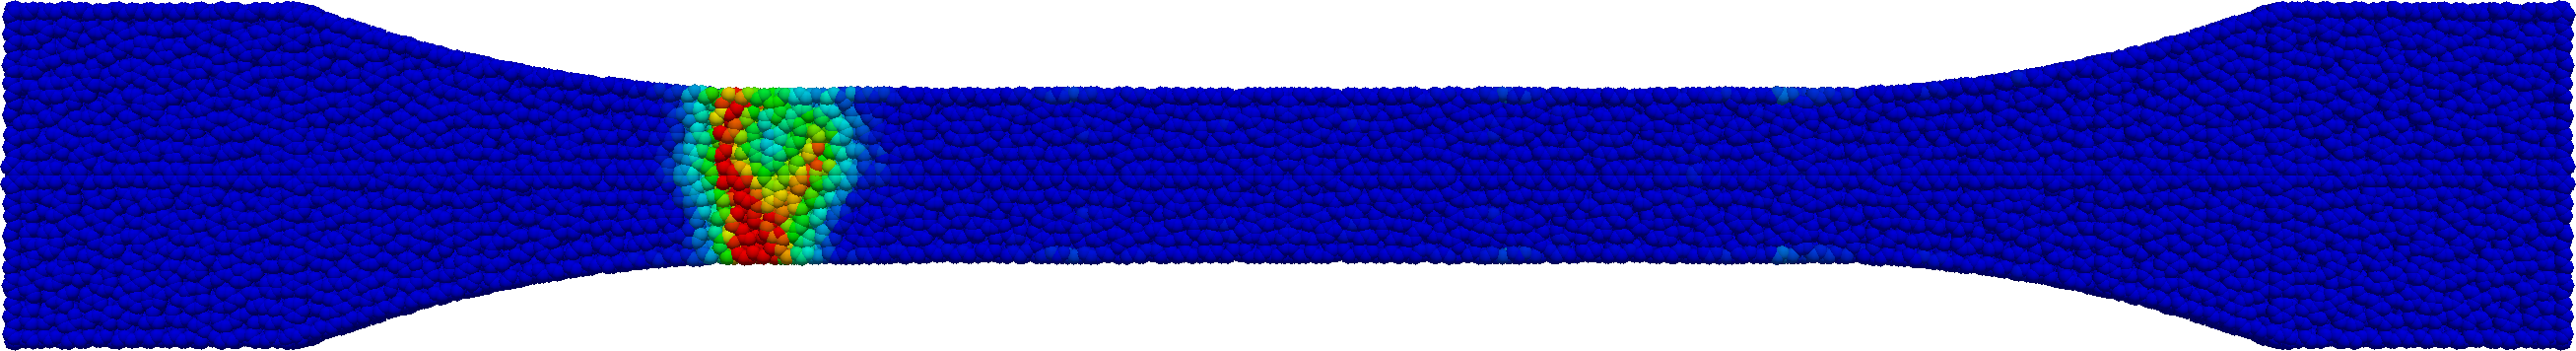
\includegraphics[angle=90,width=\linewidth,height=\figheight,keepaspectratio]{PD_Tet_Damage_0-5_1-5_1830_-z_ct.png}};
              \begin{scope}[
                shift={(PDTet2.south west)},
                x={(PDTet2.south east)},
                y={(PDTet2.north west)},
              ]
                \coordinate (spypointpdtet2) at (0.5,0.300);
                \coordinate (spyviewerpdtet2) at (1.0,0.5);
                \spy on (spypointpdtet2) in node[anchor=west] at (spyviewerpdtet2);
              \end{scope}
            \end{tikzpicture}\\
            \tikzexternaldisable
            $\delta=\SI{1.5}{\milli\meter}$
          \end{minipage}
        %}
      \end{block}
    }
  \end{column}
\end{columns}

\end{frame}